% This is a modified version of Springer's LNCS template suitable for anonymized MICCAI 2025 main conference submissions. 
% Original file: samplepaper.tex, a sample chapter demonstrating the LLNCS macro package for Springer Computer Science proceedings; Version 2.21 of 2022/01/12

\documentclass[runningheads]{llncs}
%
\usepackage[T1]{fontenc}
% T1 fonts will be used to generate the final print and online PDFs,
% so please use T1 fonts in your manuscript whenever possible.
% Other font encodings may result in incorrect characters.
%
\usepackage{graphicx,verbatim}
% Used for displaying a sample figure. If possible, figure files should
% be included in EPS format.
%
% If you use the hyperref package, please uncomment the following two lines
% to display URLs in blue roman font according to Springer's eBook style:
%\usepackage{color}
%\renewcommand\UrlFont{\color{blue}\rmfamily}
%\urlstyle{rm}
%
\begin{document}
%
\title{RetroScope: An Open Platform for Motorizing and Digitizing Vintage Microscopes}
\titlerunning{RetroScope}
% If the paper title is too long for the running head, you can set
% an abbreviated paper title here
%
\begin{comment}  %% Removed for anonymized MICCAI submission
\author{First Author\inst{1}\orcidID{0000-1111-2222-3333} \and
Second Author\inst{2,3}\orcidID{1111-2222-3333-4444} \and
Third Author\inst{3}\orcidID{2222--3333-4444-5555}}
%
\authorrunning{F. Author et al.}
% First names are abbreviated in the running head.
% If there are more than two authors, 'et al.' is used.
%
\institute{Princeton University, Princeton NJ 08544, USA \and
Springer Heidelberg, Tiergartenstr. 17, 69121 Heidelberg, Germany
\email{lncs@springer.com}\\
\url{http://www.springer.com/gp/computer-science/lncs} \and
ABC Institute, Rupert-Karls-University Heidelberg, Heidelberg, Germany\\
\email{\{abc,lncs\}@uni-heidelberg.de}}

\end{comment}

\author{Anonymized Authors}  %% Added for anonymized MICCAI submission
\authorrunning{Anonymized Author et al.}
\institute{Anonymized Affiliations \\
    \email{email@anonymized.com}}
  
\maketitle              % typeset the header of the contribution
%
\begin{abstract}
Many optical microscopes remain mechanically and optically useful for decades, even when they no longer
match the digital and automated workflows expected in modern laboratories or teaching environments. Replacing such instruments can be expensive and wasteful. This paper presents RetroScope, an open retrofit platform that motorizes and digitizes a vintage optical microscope while preserving the existing microscope body. The platform contributes a parameterized mechanical adapter strategy for coupling low-cost motors to existing focus and XY-stage controls, an embedded Raspberry Pi-based hardware and software stack, image-based calibration for pixel scale, stage scale, and backlash, and workflow-level validation through autofocus, focus stacking, and tile scanning. Rather than proposing new autofocus or stitching algorithms, these workflows are used to test whether the mechanical, electronic, calibration, and software layers work together as a usable microscopy platform. A prototype was evaluated on a vintage upright microscope using test microscopy material and no human or patient data. On the 4x objective, repeated stage-scale calibration produced 200-step standard deviations of 0.058 and 0.066 $\mu$m/step for X and Y. A hysteresis backlash model reduced the 200-step X forward error from $-204.3\pm10.8$ $\mu$m without compensation to $11.4\pm2.9$ $\mu$m. These results support RetroScope as a resource-conscious, extensible prototype for accessible microscope automation, while also showing the limits of low-cost open-loop mechanics.

\keywords{Low-resource digital pathology \and Microscope automation \and Open hardware \and Image-based calibration}
% Authors must provide keywords and are not allowed to remove this Keyword section.

\end{abstract}

\section{Introduction}

Computational pathology relies on digitized microscope images that can be stored, inspected, shared, and processed. Whole-slide scanners and integrated motorized microscopes provide this capability in many modern workflows, but their cost and hardware assumptions can limit access in teaching, small laboratories, and low-resource environments. At the same time, many older optical microscopes remain mechanically and optically useful. Their limitation is often not the lenses or frame, but the absence of motorized control, digital capture, calibrated measurement, and programmable acquisition.

Retrofit automation is therefore an attractive middle ground. Instead of replacing the microscope, a retrofit can attach motors and electronics to the manual controls that already exist. This is especially relevant for histology and pathology-adjacent education or exploratory work, where access to slide digitization can be more important than the absolute throughput of a commercial whole-slide scanner. The approach also connects to open scientific hardware, where shared designs and low-cost components can improve accessibility and reproducibility \cite{pearce2012openhardware,baden2015openlabware}.

The challenge is that a microscope retrofit is not merely a motor bracket. A useful platform must adapt to microscope-specific geometry, drive controls that were designed for humans, account for open-loop stepper motion and backlash, capture images, store metadata, and expose workflows that are useful to an operator. Low-cost mechanics also make accuracy conditional: motor steps must be related to specimen-plane displacement through calibration, and motion compensation must be evaluated under realistic workflow conditions.

This paper presents RetroScope, an open platform for motorizing and digitizing vintage microscopes. The contribution is an integrated retrofit artifact rather than a new image-analysis algorithm. The main contributions are:
\begin{enumerate}
    \item A parameterized adapter for focus knobs, XY-stage knobs, camera ports, and mounting points.
    \item A low-cost embedded hardware and software stack for live imaging, manual control, capture management, and automation.
    \item Image-based calibration and a hysteresis backlash-compensation model for making open-loop motion useful.
    \item Workflow validation through autofocus, focus stacking, and tile scanning across multiple objective profiles.
\end{enumerate}
The implementation and design artifacts are available at: \\
\textit{https://github.com/DeepMicroscopy/RetroScope}.

\section{Related Work}

Open and low-cost microscopy platforms have shown that scientific imaging hardware can be made more accessible. Foldscope demonstrates extreme-cost optical access through simplified fabrication \cite{cybulski2014foldscope}, while the OpenFlexure Microscope demonstrates low-cost robotic microscopy using 3D-printed structures and open hardware \cite{collins2020openflexure}. Open labware and 3D-printable optics work similarly argues that shared mechanical designs can reduce barriers to scientific instrumentation \cite{baden2015openlabware,zhang2013opensourceoptics}.

RetroScope differs from full open-hardware microscope designs because it keeps the existing microscope as the optical and mechanical core. The design problem is therefore adaptation rather than replacement. Commercial microscope control systems and open software controllers such as Micro-Manager and Pycro-Manager enable flexible acquisition when compatible motorized hardware is available \cite{edelstein2014advanced,pinkard2021pycromanager}. A retrofit must instead create motorized behavior through manual controls, with lower precision and stronger dependence on calibration.

Digital microscopy also requires metadata and interoperability. The Open Microscopy Environment data model and OME-TIFF format support structured biological image metadata \cite{goldberg2005ome,linkert2010metadata}. This is important for microscopy capture because objective magnification, pixel scale, stage position, focus position, and workflow type affect the meaning of the images. Finally, autofocus and tiled acquisition are well-studied microscopy workflows \cite{pech2000diatom,sun2004autofocusing,preibisch2009globally}. In RetroScope they are used as validation tasks for the platform rather than as novel algorithms.

\section{RetroScope Platform}

\subsection{Reusable Microscope Interfaces}

Many upright microscopes expose similar operator-facing interfaces: fine and coarse focus controls, XY-stage knobs, a stable frame or base, illumination controls, and a camera or observation path. RetroScope uses these recurring interfaces as the abstraction layer for the retrofit. The platform does not assume access to the internal stage or focus mechanism. It only assumes that the existing controls for humans can be coupled, measured, and calibrated.

\begin{figure}[h]
    \centering
    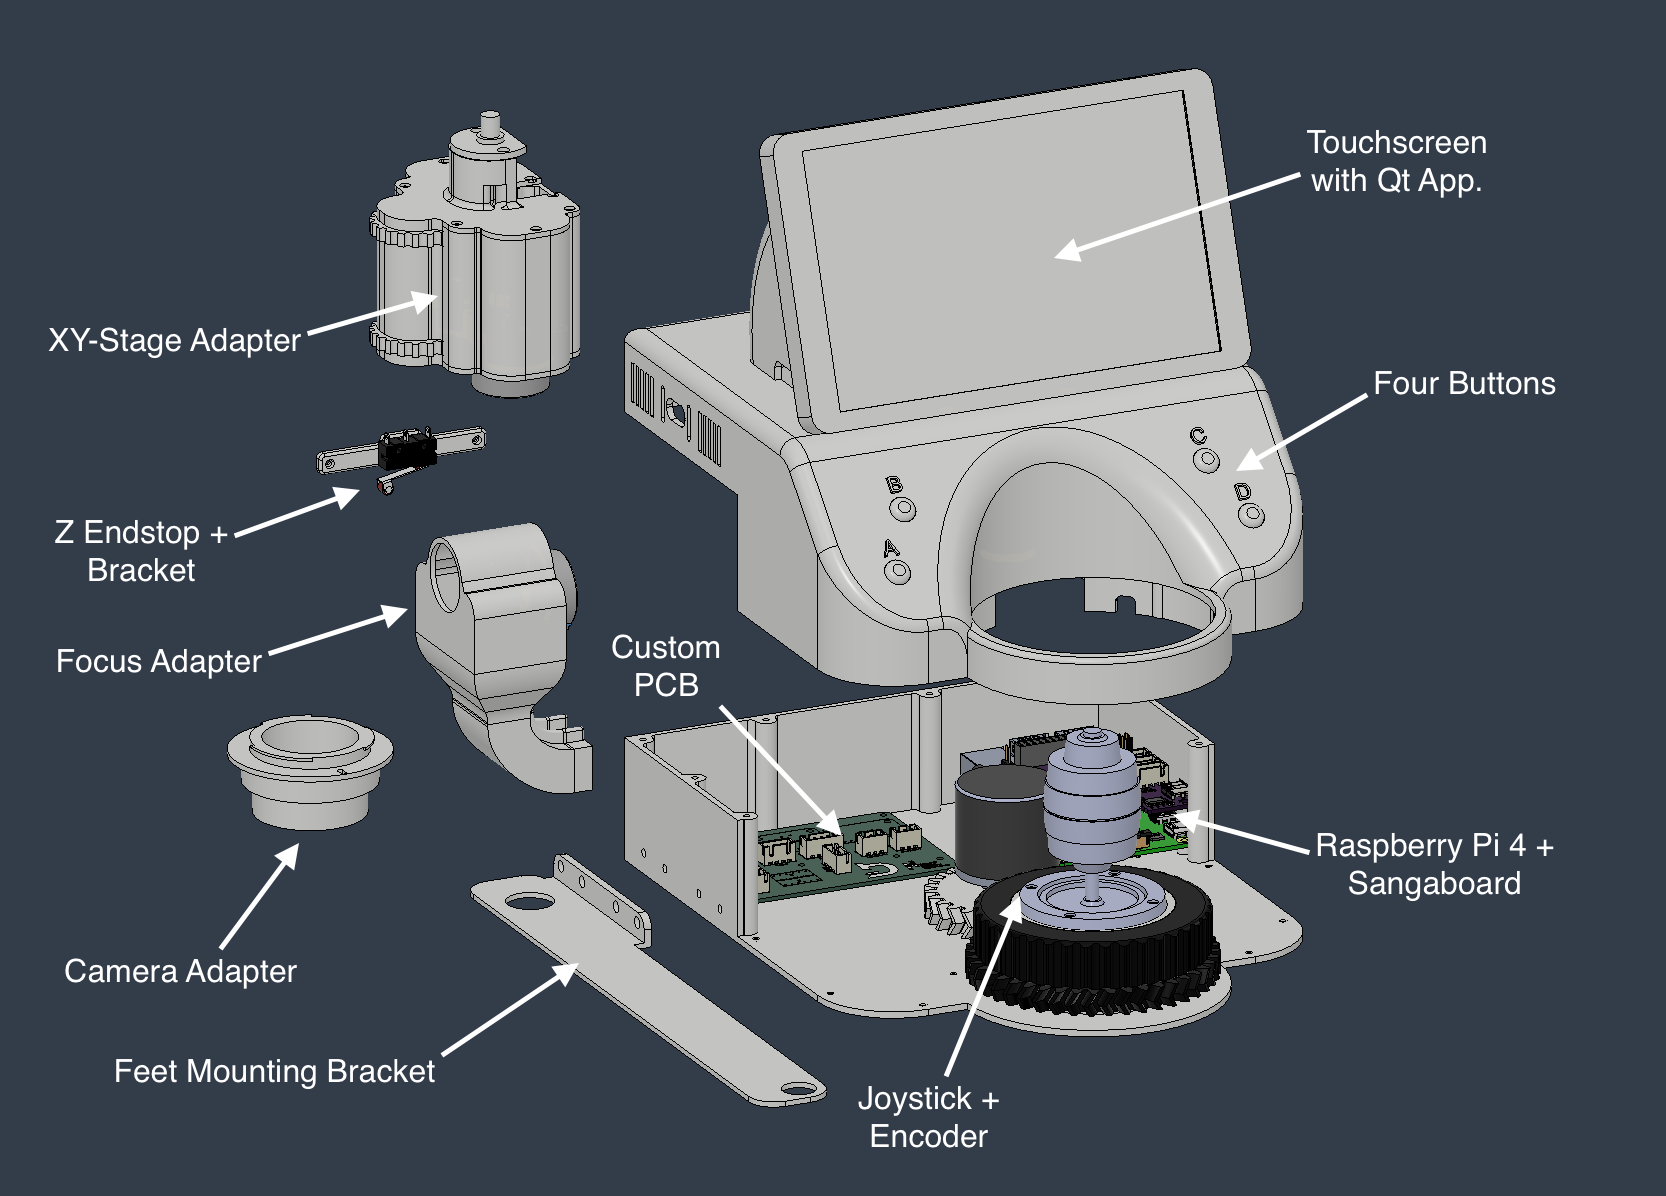
\includegraphics[width=0.9\linewidth]{figures/explode_notes.png}
    \caption[Exploded view of retrofit components]{Exploded render of the RetroScope prototype. The view separates the printed enclosure, joystick and encoder assembly, Raspberry Pi and Sangaboard electronics, custom PCB, feet mounting bracket, focus adapter, Z endstop bracket, XY-stage adapter, and camera adapter.}
    \label{fig:explode-diagram}
\end{figure}

This distinction matters for universal adaptation. A single fixed printed part cannot fit various microscope bodies, because knob diameters, axis spacing, mounting points, and optical ports vary. RetroScope therefore makes the interface configurable: the parametric model exposes focus-axis height, focus-axis radius, adapter offsets, and mounting-hole geometry as editable parameters. The same platform concept can then be regenerated for a different body dimension.

\begin{figure}[h]
\centering
\begin{tabular}{@{}cc@{}}
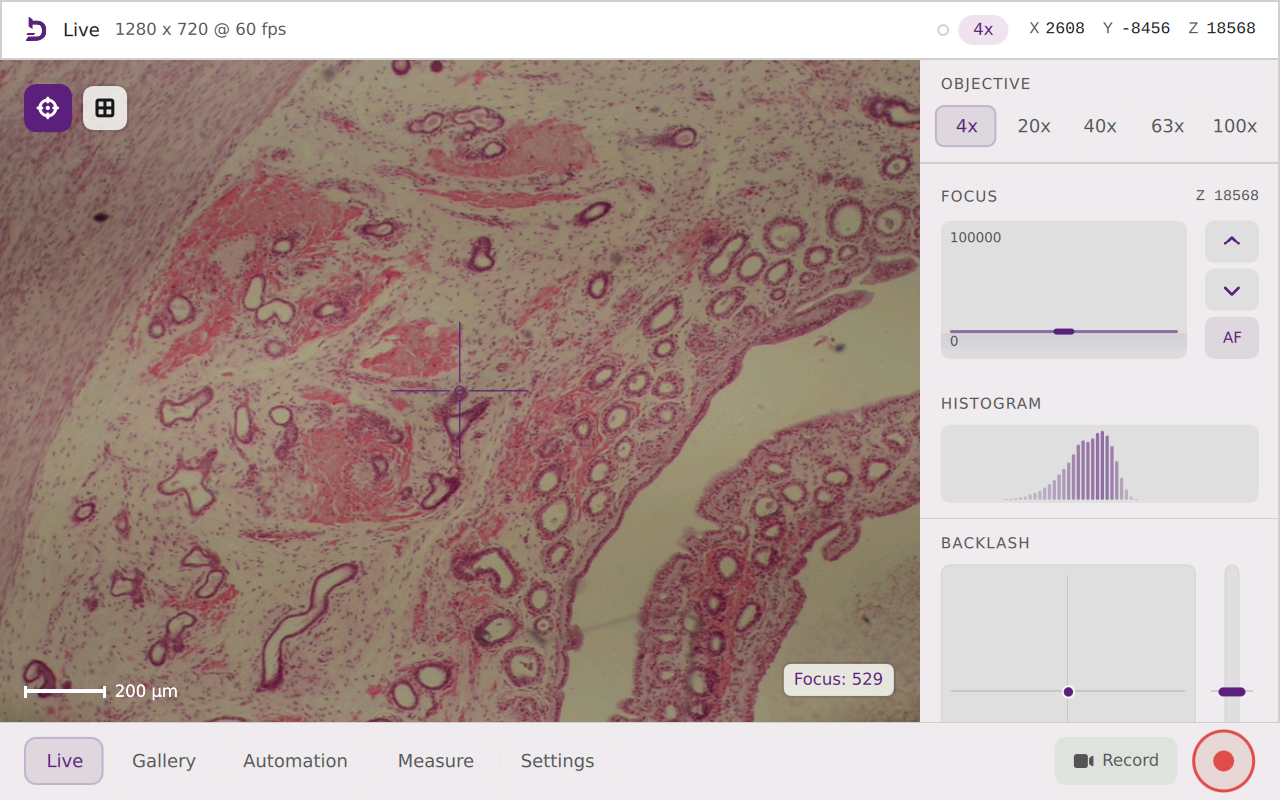
\includegraphics[width=0.5\textwidth]{figures/ui_live_view.png} &
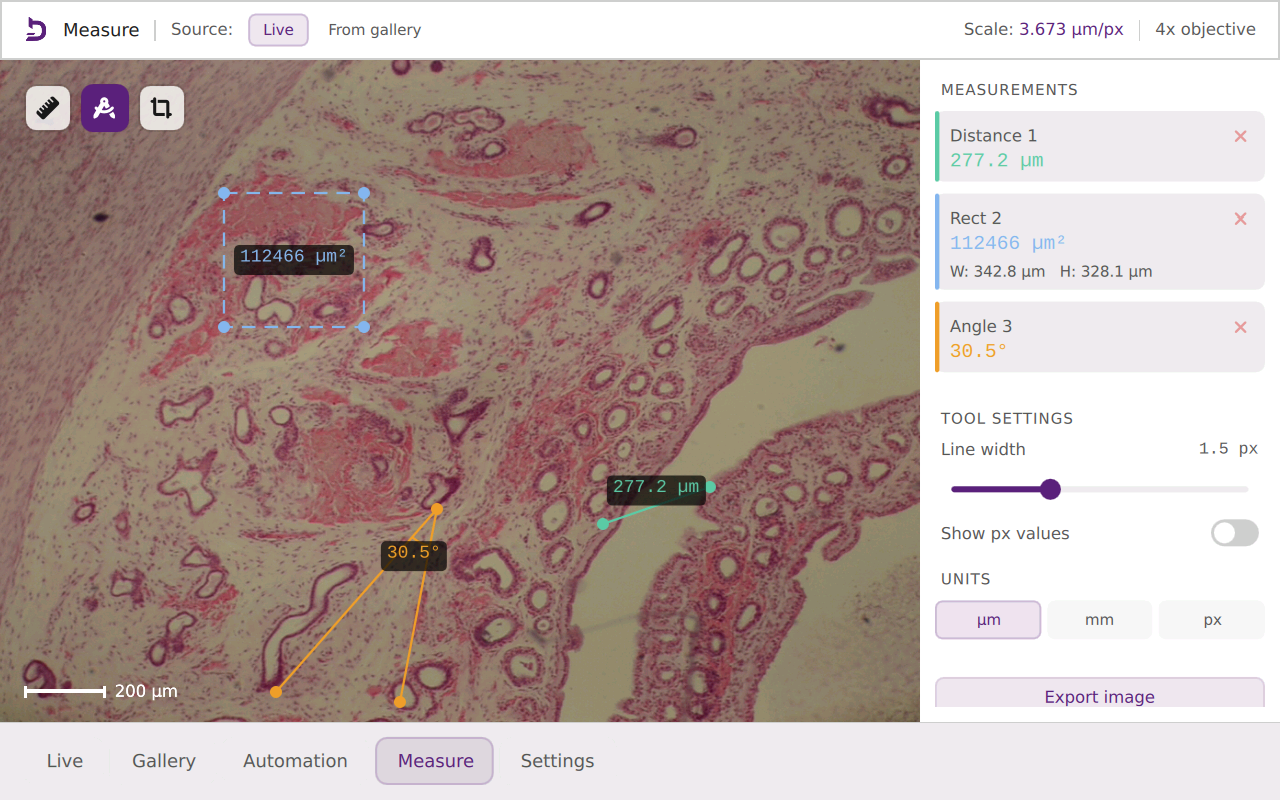
\includegraphics[width=0.5\textwidth]{figures/ui_measurements.png} \\
{\small (a) The live-view interface.} &
{\small (b) The measurement interface.}
\end{tabular}
\caption{Two examples of the RetroScope's touch interface: The live view provides camera preview, objective state, and motion controls, while the measurement view shows how, after calibration, images can be inspected with distance, area, and angle tools.}
\label{fig:ui-interfaces}
\end{figure}

\subsection{Mechanical and Embedded Design}

The prototype was built around a vintage upright microscope (Nikon Optiphot 66). The focus axis is driven by directly coupling a motor to the fine-focus axle through a printed shaft adapter. The coarse focus remains untouched. The XY stage uses a compact printed gearbox because the X and Y knobs are stacked and have different diameters. Printed gears are placed on top of the existing knobs. Motor gears and auxiliary manual knobs interface with them. The selected 12:24 tooth relation provides a 1:2 reduction, increasing torque and effective step resolution at the cost of additional gear backlash.

\begin{figure}[h]
\centering
\begin{tabular}{cc}
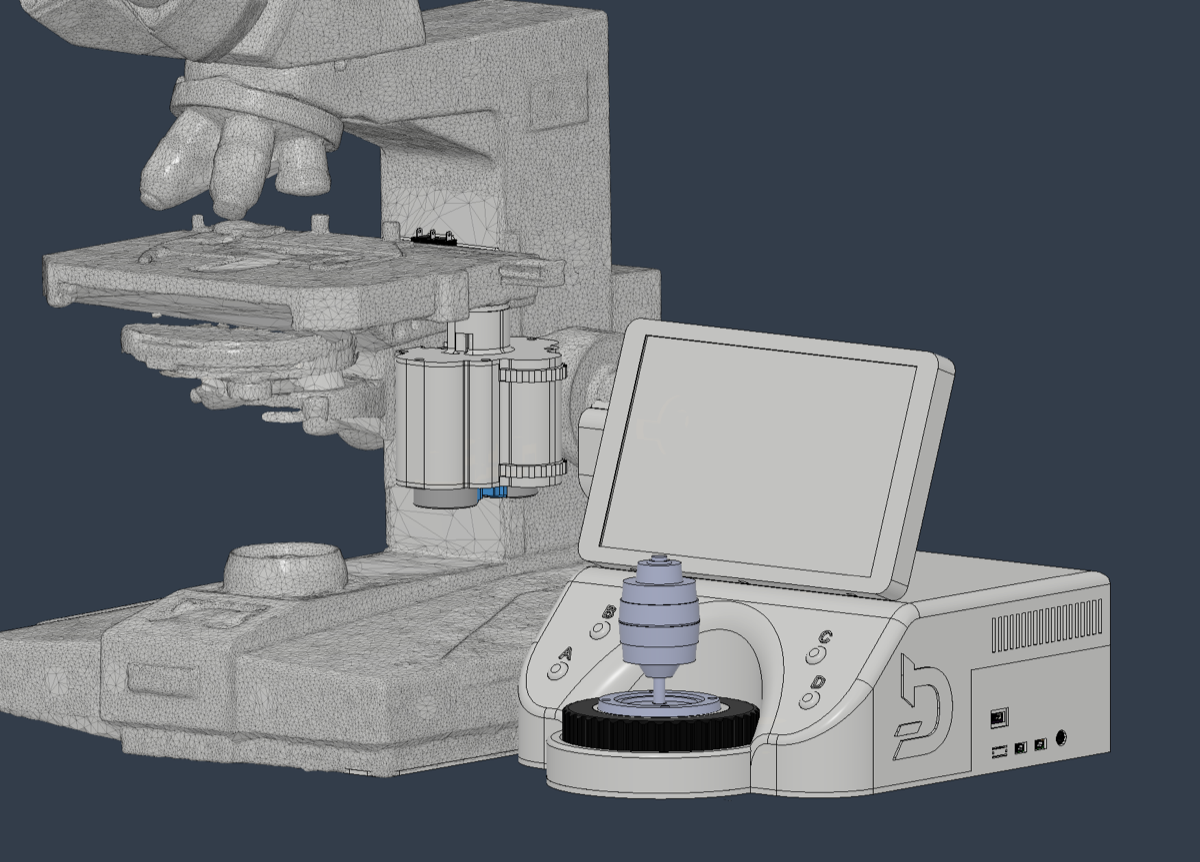
\includegraphics[width=0.5\textwidth]{figures/platform_render.png} &
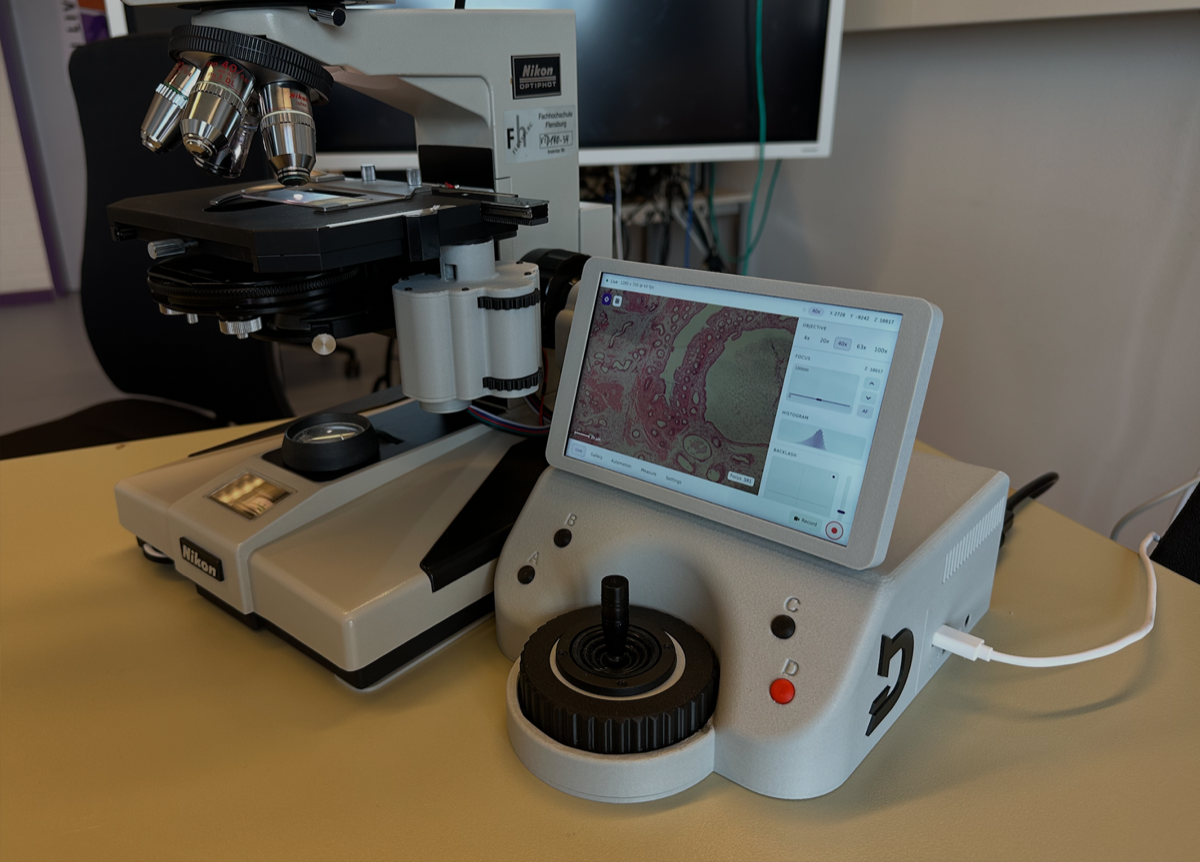
\includegraphics[width=0.5\textwidth]{figures/platform_prototype.png} \\
{\small (a) CAD render and microscope 3d scan.} &
{\small (b) Full assembled prototype.}
\end{tabular}
\caption{RetroScope retrofits an existing microscope rather than replacing it. The CAD model captures the adapter geometry and the physical prototype attaches motors, electronics, and touch display to the baseline microscope (Nikon Optiphot 66).}
\label{fig:platform}
\end{figure}

The embedded platform combines a Raspberry Pi, touchscreen, camera capture device, Sangaboard stepper controller \cite{collins2020openflexure}, low-cost 28BYJ-48 stepper motors, joystick, rotary encoder, endstop, and a custom PCB. The application is implemented in Python with PySide6/QML. It separates hardware drivers, services, domain logic, and QML bridges. The operator can use a live-view interface, joystick controls, gallery, calibration wizards, automation workflows, and a REST API for capture access and selected actions like autofocus.

\subsection{Calibration and Motion Compensation}

Calibration turns motorized motion into microscope-relevant motion. RetroScope stores objective profiles with pixel scale, stage scale, numerical aperture, focus parameters, and backlash values. Pixel-scale calibration maps image pixels to specimen-plane micrometers. Stage-scale calibration maps motor steps to X/Y displacement. These two mappings are required for measurement and tile planning because image overlap must be translated into motor steps.

The system remains open-loop: it estimates position from motor commands, not from measured stage encoders. This makes backlash compensation central. Low-cost geared steppers are attractive for accessible hardware but introduce mechanical slack and other open-loop limitations \cite{acarnley2002stepping}. RetroScope uses a per-axis hysteresis model. For axis $i$, a configured backlash width $b_i$ and slack estimate $s_i$ are maintained with
\[
    -b_i/2 \leq s_i \leq b_i/2
\]
For a compensated requested move $d_i$, the controller computes the slack take-up
\[
    p_i = \mathrm{sign}(d_i)b_i/2 - s_i
\]
and sends a single motor command
\[
    m_i = d_i + p_i
\]
After the command is accepted, the slack estimate is set to the band edge in the commanded direction. Raw moves can still update the slack estimate without applying compensation. X/Y backlash parameters are obtained through a calibration workflow that compares camera crops before and after direction reversal using image displacement measurement. Phase-correlation style registration is a standard basis for such subpixel displacement measurements \cite{guizar2008subpixel}.

\section{Workflow Validation}

RetroScope implements autofocus, focus stacking, and tile scanning. These are not claimed as new algorithms. Instead, they are validation workflows because each one exercises multiple layers of the platform.

Autofocus moves the Z axis through a configured search range, evaluates image sharpness from the camera stream, and refines the final focus position based on the highest-scoring samples. It validates Z motion, focus scoring, objective-specific parameters, and blocking movement. Focus stacking captures a sequence of Z planes and produces a blended result while preserving source images and metadata. It validates calibrated Z stepping, metadata, and gallery storage. Tile scanning captures adjacent fields of views as either a stitched panorama or a deterministic grid mosaic. It validates pixel scale, stage scale, backlash handling, capture timing, and scan planning. Dark tile seams remain visible in some outputs, likely due to illumination fall-off, vignetting, or other optical-path effects. Reducing this would require flat-field correction \cite{bowman2019flatfield}.

\begin{figure}[h]
\centering
\begin{tabular}{ccc}
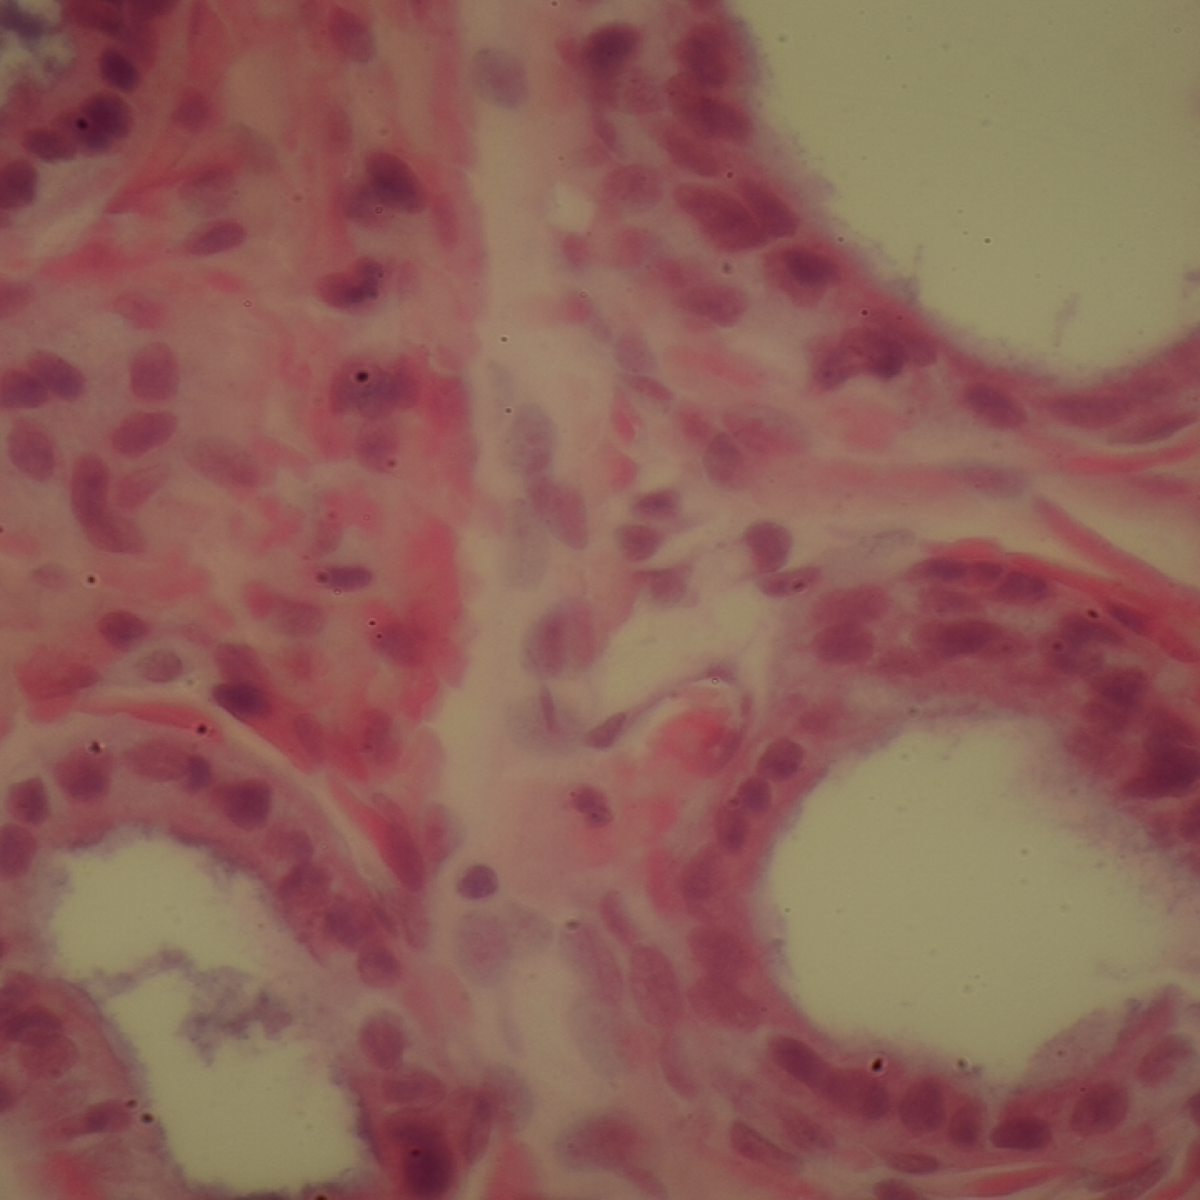
\includegraphics[width=0.364\textwidth]{figures/focus_stack_blended.png} &
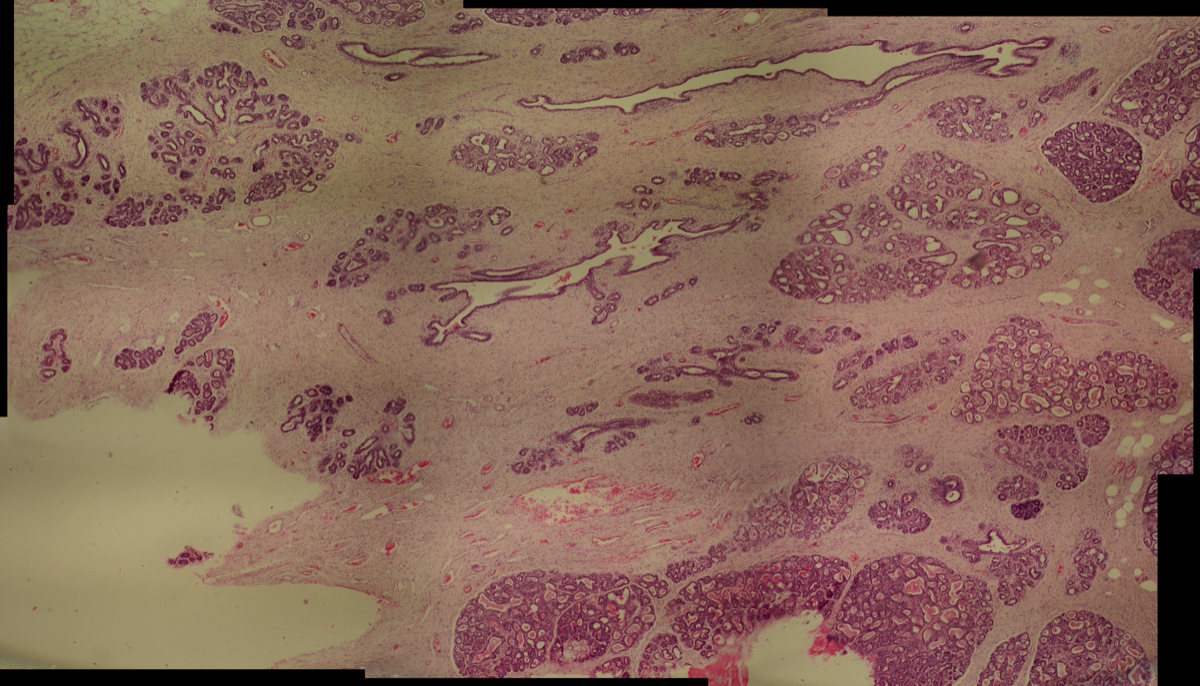
\includegraphics[width=0.636\textwidth]{figures/tile_scan_stitched.png} \\
{\small (a) Focus-stack blend.} & {\small (b) Stitched tile scan.}
\end{tabular}
\caption{Workflow examples used to validate the integrated platform. The examples demonstrate coordinated Z motion and capture for focus stacking, and calibrated XY motion and capture for tile scanning.}
\label{fig:workflows}
\end{figure}

\section{Evaluation}

\subsection{Setup}

The evaluation used the complete prototype: printed adapters, embedded electronics, custom PCB, Sangaboard-controlled motors, motion controller, calibration workflows, and automated workflows. No human data, patient data, or private clinical dataset was used. Experiments used calibration and test microscopy material to evaluate the platform behavior, not clinical diagnostic performance.

Four experiments were considered. Stage-scale repeatability measured how consistently motor steps mapped to specimen-plane movement. Motion accuracy compared uncompensated motion, an sign-based compensation mode, and the hysteresis model. Calibration repeatability repeated selected calibration measurements. Workflow reliability ran autofocus, focus stacking, and tile scanning ten times for each available objective profile.

\subsection{Motion and Calibration Results}

Table~\ref{tab:motion} summarizes the main 4x objective results. Stage-scale estimates differed between axes, confirming that separate X/Y calibration is required. In the 200-step condition, stage-scale standard deviations were 0.058 $\mu$m/step for X and 0.066 $\mu$m/step for Y. Motion results show the strongest improvement for X at 200 steps: the hysteresis model reduced mean forward error from $-204.3$ $\mu$m without compensation to $11.4$ $\mu$m. The Y axis improved less cleanly and retained a larger reversal residual, because the 3d printed gears on the Y axis has a longer distance between motor and the knob, causing addtional flex by bending plastic. The 100-step conditions were less stable because the commanded displacement was close to or below the configured backlash width.

\begin{table}[h]
\caption{Selected 4x motion and calibration results. Values are mean $\pm$ standard deviation across ten valid trials.}
\label{tab:motion}
\centering
\small
\setlength{\tabcolsep}{6pt}
\begin{tabular}{llll}
\hline
Experiment & Axis/condition & Quantity & Result \\
\hline
Stage scale & X, 200 steps & $\mu$m/step & $2.223\pm0.058$ \\
Stage scale & Y, 200 steps & $\mu$m/step & $3.136\pm0.066$ \\
Calibration repeat & X stage scale & $\mu$m/step & $2.232\pm0.070$ \\
Calibration repeat & Y stage scale & $\mu$m/step & $3.148\pm0.110$ \\
Calibration repeat & X backlash residual & $\mu$m & $2.150\pm1.385$ \\
Calibration repeat & Y backlash residual & $\mu$m & $1.611\pm1.464$ \\
Motion, no comp. & X, 200 steps & forward error & $-204.3\pm10.8$ $\mu$m \\
Motion, sign comp. & X, 200 steps & forward error & $-30.4\pm58.5$ $\mu$m \\
Motion, hysteresis & X, 200 steps & forward error & $11.4\pm2.9$ $\mu$m \\
Motion, no comp. & Y, 200 steps & forward error & $-260.1\pm18.5$ $\mu$m \\
Motion, sign comp. & Y, 200 steps & forward error & $-60.6\pm83.0$ $\mu$m \\
Motion, hysteresis & Y, 200 steps & forward error & $-35.8\pm16.4$ $\mu$m \\
\hline
\end{tabular}
\end{table}

\subsection{Workflow Reliability}

Table~\ref{tab:workflow} reports workflow reliability. All 120 workflow trials completed successfully: autofocus, focus stacking, and tile scanning each completed 10/10 repetitions for 4x, 20x, 40x, and 63x objective profiles. Autofocus duration was recorded. Focus-stacking and tile-scanning durations were not recorded in this evaluation. The 4x autofocus duration was longer because the low-magnification profile used a larger search range.

\begin{table}[h]
\caption{Workflow reliability across objective profiles. Autofocus duration is mean $\pm$ standard deviation over ten successful runs.}
\label{tab:workflow}
\centering
\small
\setlength{\tabcolsep}{6pt}
\begin{tabular}{lcccc}
\hline
Objective & Autofocus & Focus stack & Tile scan & AF duration (s) \\
\hline
4x  & 10/10 & 10/10 & 10/10 & $59.84\pm0.49$ \\
20x & 10/10 & 10/10 & 10/10 & $17.59\pm0.31$ \\
40x & 10/10 & 10/10 & 10/10 & $14.66\pm0.17$ \\
63x & 10/10 & 10/10 & 10/10 & $14.21\pm0.07$ \\
\hline
\end{tabular}
\end{table}

\section{Discussion and Conclusion}

The results support RetroScope as a working low-cost retrofit prototype for accessible microscope automation. The platform successfully combines a parameterized mechanical adapter, embedded control hardware, modular software, image-based calibration, and workflow automation. For low-resource computational pathology, RetroScope is intended as an enabling platform rather than a diagnostic system: it helps existing microscopes become part of digital and automated workflows without requiring full instrument replacement.

The evaluation also bounds the claims. RetroScope is not a precision stage and does not replace a clinical whole-slide scanner. It controls a chain of existing microscope mechanics, printed gears, low-cost steppers, and open-loop estimates. Backlash compensation can improve predictable lost motion, but it cannot remove flex, missed steps, manual disturbances, or optical artifacts. Quantitative motion evaluation was done for a 4x objective, while workflow reliability was tested across four objective profiles. Physical adaptation was demonstrated on one microscope body and virtually through the parametric model.

Several limitations therefore remain. The prototype was physically validated on a single microscope body, so the parametric model demonstrates adaptability as a design principle but not yet as a broad empirical claim across microscope families. The system also tracks commanded motor position rather than measured sample position, which means that calibration can become invalid after manual stage movement, loosened printed parts, changed friction, or missed steps. Finally, the workflow evaluation measured successful completion rather than diagnostic image quality, focus-stack quality, or tile-alignment accuracy. These gaps are important because low-resource deployment depends not only on whether a scan can be completed, but also on whether the resulting data is stable enough for the intended use.

Nevertheless, the prototype demonstrates that vintage microscopes can be extended into programmable digital imaging systems without discarding the original optical instrument. Autofocus, focus stacking, and tile scanning serve as integrated validation tasks showing that calibration and compensation are sufficient for repeated automated operation under the tested conditions. Future work should add closed-loop sensing, physical validation on additional microscope bodies, flat-field correction for tile scans, and more detailed workflow quality metrics.

\newpage

%
% ---- Bibliography ----
%
% BibTeX users should specify bibliography style 'splncs04'.
% References will then be sorted and formatted in the correct style.
%
% \bibliographystyle{splncs04}
% \bibliography{mybibliography}
%
\begin{thebibliography}{8}
\bibitem{pearce2012openhardware}
Pearce, J.M.: Building research equipment with free, open-source hardware. Science \textbf{337}(6100), 1303--1304 (2012). \doi{10.1126/science.1228183}

\bibitem{baden2015openlabware}
Baden, T., Chagas, A.M., Gage, G., Marzullo, T., Prieto-Godino, L.L., Euler, T.: Open labware: 3-D printing your own lab equipment. PLOS Biology \textbf{13}(3), e1002086 (2015). \doi{10.1371/journal.pbio.1002086}

\bibitem{cybulski2014foldscope}
Cybulski, J.S., Clements, J., Prakash, M.: Foldscope: Origami-based paper microscope. PLOS ONE \textbf{9}(6), e98781 (2014). \doi{10.1371/journal.pone.0098781}

\bibitem{collins2020openflexure}
Collins, J.T., Knapper, J., Stirling, J., et al.: Robotic microscopy for everyone: the OpenFlexure Microscope. Biomedical Optics Express \textbf{11}(5), 2447--2460 (2020). \doi{10.1364/BOE.385729}

\bibitem{zhang2013opensourceoptics}
Zhang, C., Anzalone, N.C., Faria, R.P., Pearce, J.M.: Open-source 3D-printable optics equipment. PLOS ONE \textbf{8}(3), e59840 (2013). \doi{10.1371/journal.pone.0059840}

\bibitem{edelstein2014advanced}
Edelstein, A.D., Tsuchida, M.A., Amodaj, N., Pinkard, H., Vale, R.D., Stuurman, N.: Advanced methods of microscope control using Micro-Manager software. Journal of Biological Methods \textbf{1}(2), e10 (2014). \doi{10.14448/jbm.2014.36}

\bibitem{pinkard2021pycromanager}
Pinkard, H., Stuurman, N., Ivanov, I.E., et al.: Pycro-Manager: open-source software for customized and reproducible microscope control. Nature Methods \textbf{18}, 226--228 (2021). \doi{10.1038/s41592-021-01087-6}

\bibitem{goldberg2005ome}
Goldberg, I.G., Allan, C., Burel, J.M., et al.: The Open Microscopy Environment (OME) Data Model and XML file: open tools for informatics and quantitative analysis in biological imaging. Genome Biology \textbf{6}(5), R47 (2005). \doi{10.1186/gb-2005-6-5-r47}

\bibitem{linkert2010metadata}
Linkert, M., Rueden, C.T., Allan, C., et al.: Metadata matters: access to image data in the real world. Journal of Cell Biology \textbf{189}(5), 777--782 (2010). \doi{10.1083/jcb.201004104}

\bibitem{pech2000diatom}
Pech-Pacheco, J.L., Cristobal, G., Chamorro-Martinez, J., Fernandez-Valdivia, J.: Diatom autofocusing in brightfield microscopy: a comparative study. In: Proceedings 15th International Conference on Pattern Recognition, vol. 3, pp. 314--317 (2000). \doi{10.1109/ICPR.2000.903548}

\bibitem{sun2004autofocusing}
Sun, Y., Duthaler, S., Nelson, B.J.: Autofocusing in computer microscopy: selecting the optimal focus algorithm. Microscopy Research and Technique \textbf{65}(3), 139--149 (2004). \doi{10.1002/jemt.20118}

\bibitem{preibisch2009globally}
Preibisch, S., Saalfeld, S., Tomancak, P.: Globally optimal stitching of tiled 3D microscopic image acquisitions. Bioinformatics \textbf{25}(11), 1463--1465 (2009). \doi{10.1093/bioinformatics/btp184}

\bibitem{bowman2019flatfield}
Bowman, R.W., Vodenicharski, B., Collins, J.T., Stirling, J.: Flat-field and colour correction for the Raspberry Pi camera module. Journal of Open Hardware \textbf{4}(1) (2020). \doi{10.5334/joh.20}

\bibitem{acarnley2002stepping}
Acarnley, P.P.: Stepping Motors: A Guide to Theory and Practice. 4th edn. Institution of Electrical Engineers, London (2002)

\bibitem{guizar2008subpixel}
Guizar-Sicairos, M., Thurman, S.T., Fienup, J.R.: Efficient subpixel image registration algorithms. Optics Letters \textbf{33}(2), 156--158 (2008). \doi{10.1364/OL.33.000156}

\end{thebibliography}
\end{document}
